\chapter{Kinematik}

Die Mechanik kann in die Bereiche Kinematik, Dynamik, Statik und Kinetik unterteilt werden,
wie in Abbildung \ref{fig:einteilungMechanik} gezeigt.

\begin{figure}[H]    
    \centering          %     left botm right top
    \includegraphics[clip, trim=0cm 0cm 0cm 0cm,width=.4\textwidth]{einteilungMechanik.png} %.6 stands for 0.6 x textwidth
    \caption{Einteilung Mechanik \cite{bartsch_dynamik_2023}}
    \label{fig:einteilungMechanik}
\end{figure}

Die Kinematik ist die Lehre vom geometrischen und zeitlichen Bewegungsablauf, ohne
dass auf die Kräfte als Ursache oder Wirkung der Bewegung eingegangen wird.
Ziel ist es angeben zu können an welchem Ort sich ein Körper zu welcher Zeit
befindet.

\begin{figure}[H]    
    \centering          %     left botm right top
    \includegraphics[clip, trim=0cm 0cm 0cm 0cm,width=.7\textwidth]{kinematik_darstellung_leicht.png} %.6 stands for 0.6 x textwidth
    \caption{Gleichmässige Beschleunigung - einfaches Beispiel Kinematik \cite{noauthor_mechanik_nodate}}
    \label{fig:einfBspKinem}
\end{figure}

\section{Die Reduktion auf einen Massenpunkt}

Die Reduktion der Masse eines Körpers (Bauteils) auf einen Punkt ist eine 
Vereinfachung. Man nimmt dabei an, dass sich der Körper unter dem
Einfluss von Kräften so benimmt, wie wenn seine gesamte Masse im Schwerpunkt
konzentriert wäre. Wann diese Vereinfachung zulässig ist, hängt von den relativen
Abmessungen des Körpers zu seiner Umgebung und von dessen Bewegungszustand ab \cite{bartsch_dynamik_2023}.

\section{Geradlinige Bewegung des Massenpunktes}

Die Bewegung eines Punktes wird durch die Lage (Ortsvektor $\overrightarrow{r}$), 
die Geschwindigkeit $\overrightarrow{v}$ und die Beschleunigung $\overrightarrow{a}$ beschrieben, 
wobei die folgenden Beziehungen gelten, vereinfacht für die 1-dimensionale, 
geradlinige Bewegung dargestellt:

\begin{equbox}
    \begin{minipage}{.2\textwidth}
        Lage: \\
        Geschwindigkeit: \\
        Beschleunigung:
    \end{minipage}
    \hspace{.1\textwidth}
    \begin{minipage}{.3\textwidth}
        $x(t)$ \\
        $v(t) = \dot{x}(t)$ \\
        $a(t) = \dot{v}(t) = \ddot{x}(t)$
    \end{minipage}
\end{equbox}

Bei der Verwendung eines kartesischen Koordinatensystems können für die anderen beiden
Richtungen $y$ und $z$ analoge Beziehungen aufgestellt werden.

Für spezielle Bewegungsarten können die Beziehungen zwischen den drei Grössen formell
bestimmt werden.

\subsection{Konstante Geschwindigkeit}

Abbildung \ref{fig:konstanteGeschwindigkeit} zeigt die Beziehungen zwischen $a$, $v$ und $x$ 
bei konstanter Geschwindigkeit ohne Beschleunigung. Ein Beispiel dafür ist ein Fahrzeug auf der Autobahn
bei gleichbleibender Geschwindigkeit.

\begin{equbox}
    \begin{minipage}{.3\textwidth}
        Beschleunigung: \\
        Geschwindigkeit: \\
        Lage:
    \end{minipage}
    \hspace{.1\textwidth}
    \begin{minipage}{.3\textwidth}
        $a = 0ms^{-2}$ \\
        $v(t) = konstant$ \\
        $x(t) = x_0 + v_0 \cdot t$
    \end{minipage}
\end{equbox}

\begin{figure}[H]    
    \centering          %     left botm right top
    \includegraphics[clip, trim=0cm 0cm 0cm 0cm,width=\textwidth]{konstante_geschwindigkeit_grafiken.png} %.6 stands for 0.6 x textwidth
    \caption{Keine Beschleunigung, konstante Geschwindigkeit, $v_0 = 5ms^{-1}$, $x_0 = 0m$}
    \label{fig:konstanteGeschwindigkeit}
\end{figure}

\subsection{Konstante Beschleunigung}

Der freie Fall eines Objektes ist ein typisches Beispiel für die konstante Beschleunigung.
Dabei ist die Gravitation $g$ die Beschleunigung: $a = g = 9.81ms^{-2}$.

\begin{equbox}
    \begin{minipage}{.3\textwidth}
        Beschleunigung: \\
        Geschwindigkeit: \\
        Lage: \\
        Es gilt (wenn a = konst.):
    \end{minipage}
    \hspace{.1\textwidth}
    \begin{minipage}{.3\textwidth}
        $a = konstant$ \\
        $v(t) = v_0 + a \cdot t$ \\
        $x(t) = x_0 + v_0 \cdot t + \frac{1}{2} \cdot a \cdot t^2$ \\
        $v^2 = 2 \cdot a \cdot (x - x_0) + v_0^2$
    \end{minipage}
\end{equbox}

\begin{bspbox}
    \begin{minipage}{.58\textwidth}

        Ein Ball wird von einer Höhe $h = y_0 = 200m$ fallen gelassen. Mit $g$ und $h$ können 
        alle weiteren Grössen wie die Lage und Geschwindigkeit
        zu jedem beliebigen Zeitpunkt berechnet werden. 
        Wenn wir die Aufprallgeschwindigkeit berechnen 
        möchten (der Luftwiderstand wird hier vernachlässigt):

        Geg: $y_0 = 200m$, $g = -9.81ms^{-2}$, $v_0 = 0ms^{-1}$
    \end{minipage}
    \hspace{.05\textwidth}
    \begin{minipage}{.37\textwidth}
        \begin{figure}[H]   
            \centering          %     left botm right top
            \includegraphics[clip, trim=0cm 0cm 0cm 0cm,width=\textwidth]{freier_fall-3100070738.jpg} %.6 stands for 0.6 x textwidth
            \label{fig:freierfall}
        \end{figure}
    \end{minipage}

    \begin{minipage}[t]{.48\textwidth}
        Fallzeit $t$:
        \begin{align*}
            y(t) &= y_0 + v_0 \cdot t + \frac{1}{2} \cdot g \cdot t^2 \\
            0m &= 200m + 0ms^{-1} \cdot t + \frac{1}{2} \cdot (-9.81ms^{-2}) \cdot t^2 \\
            -200m &= \frac{1}{2} \cdot (-9.81ms^{-2}) \cdot t^2 \\
            200m &= \frac{1}{2} \cdot 9.81ms^{-2} \cdot t^2 \\
            t &= \sqrt{\frac{2 \cdot 200m}{9.81ms^{-2}}} = 6.386s
        \end{align*}
    \end{minipage}
    \hspace{.04\textwidth}
    \begin{minipage}[t]{.48\textwidth}
        Aufprallgeschwindigkeit v:
        \begin{align*}
            v^2 &= 2 \cdot g \cdot (y - y_0) + v_0^2 \\
            v^2 &= 2 \cdot (-9.81ms^{-2}) \cdot (0m - 200m) + 0ms^{-1} \\
            v^2 &= 2 \cdot (-9.81ms^{-2}) \cdot (-200m) \\
            v^2 &= 2 \cdot 9.81ms^{-2} \cdot 200m \\
            v &= \sqrt{2 \cdot 9.81ms^{-2} \cdot 200m} \\
            v &= 62.64ms^{-1}
        \end{align*}
    \end{minipage}

    \begin{figure}[H]    
        \centering          %     left botm right top
        \includegraphics[clip, trim=0cm 0cm 0cm 0cm,width=.9\textwidth]{freier_fall_ball200.png} %.6 stands for 0.6 x textwidth
        \caption{$a$, $v$ und $y$, Ball im freien Fall}
        \label{fig:ballImFreienFall}
    \end{figure}
\end{bspbox}

\subsection{Beliebige Beschleunigung}

Wir wissen, dass:

\begin{minipage}{.2\textwidth}
    Lage: \\
    Geschwindigkeit: \\
    Beschleunigung:
\end{minipage}
\hspace{.1\textwidth}
\begin{minipage}{.3\textwidth}
    $x(t)$ \\
    $v(t) = \dot{x}(t)$ \\
    $a(t) = \dot{v}(t) = \ddot{x}(t)$
\end{minipage}

Durch diese Beziehungen können für alle geradlinigen Bewegungen aus der 
Beschleunigung die Geschwindigkeit und Lage einer Masse berechnet werden wenn die 
Anfangsbedingungen $v_0$ und $x_0$ bekannt sind. 

\begin{bspbox}
    Abbildung \ref{fig:beliebigeBeschleunigung}
    zeigt ein Beispiel für $a = sin(t)$, $v_0 = 0ms^{-1}$ und $x_0 = 0m$.

    \begin{figure}[H]    
        \centering          %     left botm right top
        \includegraphics[clip, trim=0cm 0cm 0cm 0cm,width=\textwidth]{beliebige_beschleunigung.png} %.6 stands for 0.6 x textwidth
        \caption{$a$, $v$ und $x$ für $a = sin(t)$, $v_0 = 0ms^{-1}$ und $x_0 = 0m$ }
        \label{fig:beliebigeBeschleunigung}
    \end{figure}

    \begin{align*}
        v(t) &= \int a(t) \, dt = \int \sin(t) \, dt = -\cos(t) + C \\
        v(0) &= 0 \implies 0 = -\cos(0) + C \implies C = 1 \\
        v(t) &= 1 - \cos(t) \\
        \\
        x(t) &= \int v(t) \, dt = \int (1 - \cos(t)) \, dt = t - \sin(t) + D \\
        x(0) &= 0 \implies 0 = 0 - \sin(0) + D \implies D = 0 \\
        x(t) &= t - \sin(t)
    \end{align*}
\end{bspbox}

\section{Die Resultierende Beschleunigung und Geschwindigkeit}

Die Geschwindigkeit $v$ und die Beschleunigung $a$ sind vektorielle Grössen. Sie können im 
kartesischen Koordinatensystem in die Richtungen $x$, $y$ und $z$ aufgeteilt werden.

Umgekehrt können die Geschwindigkeiten eines Objektes (reduziert auf den Massenpunkt) in die 
verschiedenen Richtungen zu einer Resultierenden zusammengefasst werden.

\begin{bspbox}
    Folgend ein ein Beispiel für die vektorielle Addition 
    zweier Geschwindigkeiten/ Beschleunigungen in der $x$/$y$-Ebene:

    \begin{minipage}{.48\textwidth}
        \begin{equbox}
            \begin{align*}
                \vec{v}_{\text{res}} &= \vec{v}_x + \vec{v}_y \\
                v_{\text{res}} &= \sqrt{v_x^2 + v_y^2} \\
                \tan \theta_v &= \frac{v_y}{v_x}
            \end{align*}
        \end{equbox}
        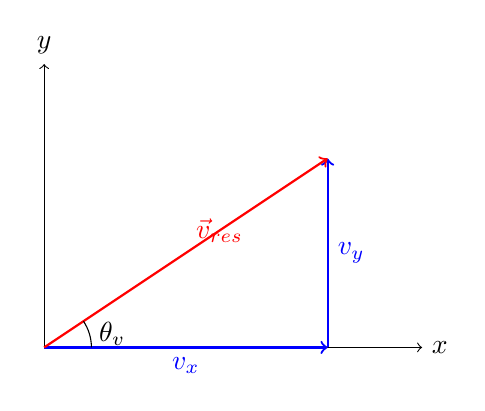
\begin{tikzpicture}[scale=1.2]
            % Achsen
            \draw[->] (0,0) -- (4,0) node[right]{$x$};
            \draw[->] (0,0) -- (0,3) node[above]{$y$};

            \draw[->, thick, blue] (0,0) -- (3,0) node[midway,below]{$v_x$};
            \draw[->, thick, blue] (3,0) -- (3,2) node[midway,right]{$v_y$};
            \draw[->, thick, red] (0,0) -- (3,2) node[midway,above right]{$\vec{v}_{\text{res}}$};

            \draw (0.5,0) arc (0:33.69:0.5) node[midway,right]{$\theta_v$};
        \end{tikzpicture}
    \end{minipage}
    \hspace{.04\textwidth}
    \begin{minipage}{.48\textwidth}
        \begin{equbox}
            \begin{align*}
                \vec{a}_{\text{res}} &= \vec{a}_x + \vec{a}_y \\
                a_{\text{res}} &= \sqrt{a_x^2 + a_y^2} \\
                \tan \theta_a &= \frac{a_y}{a_x}
            \end{align*}
        \end{equbox}
        \begin{tikzpicture}[scale=1.2]
            % Achsen
            \draw[->] (0,0) -- (4,0) node[right]{$x$};
            \draw[->] (0,0) -- (0,3) node[above]{$y$};

            % Vektoren
            \draw[->, thick, green] (0,0) -- (2,0) node[midway,below]{$a_x$};
            \draw[->, thick, green] (2,0) -- (2,1.5) node[midway,right]{$a_y$};
            \draw[->, thick, purple] (0,0) -- (2,1.5) node[midway,above right]{$\vec{a}_{\text{res}}$};

            % Winkel
            \draw (0.5,0) arc (0:36.87:0.5) node[midway,right]{$\theta_a$};
        \end{tikzpicture}
    \end{minipage}
\end{bspbox}



\section{Kreisbewegung des Massenpunktes}

Die ungleichförmige Bewegung eines Massenpunktes auf einer Kreisbahn ist ein Spezialfall
der ebenen krummlinigen Bewegung. 

\begin{figure}[H]
    \centering          %     left botm right top
    \includegraphics[width=.4\textwidth]{kreisbewegung.png}
    \caption{Kreisbeweung dargestellt \cite{noauthor_bewegung_nodate}}
    \label{fig:kreisbewegung}
\end{figure}

Der Radius ist konstant und nur die Koordinate $\phi(t)$
eine Funktion der Zeit. Damit ergeben sich die drei Bewegungsgrössen ($s$ = Umfangsweg) \cite{bartsch_dynamik_2023}:

\begin{equbox}
    \begin{minipage}{.65\textwidth}
        Lage, Winkel $\phi$: \\
        Geschwindigkeit, Winkelgeschwindigkeit $\omega$: \\
        Beschleunigung tangential, Winkelbeschleunigung $\alpha$:
    \end{minipage}
    \hspace{.1\textwidth}
    \begin{minipage}{.3\textwidth}
        $s = \phi \cdot r$ \\
        $v = \omega \cdot r$ \\
        $a_t = \alpha \cdot r$
    \end{minipage}
\end{equbox}

Analog zur geradlinigen Bewegung gelten zwischen den Bewegungsgrössen die Beziehungen:

\begin{equbox}
    \begin{minipage}{.2\textwidth}
        Winkel: \\
        Winkelgeschwindigkeit: \\
        Winkelbeschleunigung:
    \end{minipage}
    \hspace{.1\textwidth}
    \begin{minipage}{.3\textwidth}
        $\phi(t)$ \\
        $\omega(t) = \dot{\phi}(t)$ \\
        $\alpha(t) = \dot{\omega}(t) = \ddot{\phi}(t)$
    \end{minipage}
\end{equbox}

\begin{minipage}{.68\textwidth}
    Auch bei einer gleichförmigen Kreisbewegung ($v$ = const.) existiert immer
    eine Beschleunigung, die radiale Zentripetalbeschleunigung $a_r$.
    Sie ist stets gegen das Zentrum gerichtet (Abbildung \ref{fig:spezialfallKreisbewegung}).

    \begin{equbox}
        \begin{equation}
            |a_r| = \omega^2 \cdot r
        \end{equation}
    \end{equbox}
    \vspace{0.5cm}

    Bei ungleichförmiger Bewegung ($v$ nicht konst.) kommt eine
    tangentiale Komponente der Beschleunigung at dazu.

    \begin{equbox}
        \begin{equation}
            a_t = \dot{v}_t
        \end{equation}
    \end{equbox}

\end{minipage}
\hspace{.05\textwidth}
\begin{minipage}{.25\textwidth}
    \begin{figure}[H]   
        \centering          %     left botm right top
        \includegraphics[clip, trim=0cm 0cm 0cm 0cm,width=\textwidth]{spezialfall_kreisbewegung.png} %.6 stands for 0.6 x textwidth
        \caption{Spezialfall Kreisbewegung}
        \label{fig:spezialfallKreisbewegung}
    \end{figure}
\end{minipage}

\subsection{Rotationsgeschwindigkeit}

Die Winkelgeschwindigkeit $\omega$, Frequenz $f$, Drehzahl $n$ und 
Umlaufzeit $T$ beschreiben, wie schnell etwas rotiert. 

\begin{figure}[H]
    \centering          %     left botm right top
    \includegraphics[width=.2\textwidth]{rotationsgeschwindigkeit.png}
    \caption{Rotation und Grundeinheiten \cite{bartsch_dynamik_2023}}
    \label{fig:rotationsgeschwindigkeit}
\end{figure}

Je nach Anwendungsbereich
wird das Eine oder Andere verwendet, sie beschreiben allerdings genau
das Selbe und stehen im direkten Verhältnis zueinander:

\begin{equbox}
    \begin{equation}
        \omega = \frac{\phi}{t} = \frac{2 \cdot \pi}{T} = 2 \cdot \pi \cdot f = 2 \cdot \pi \cdot n
    \end{equation}
\end{equbox}

Die Einheiten sind:

\begin{minipage}{.48\textwidth}
    \begin{itemize}
        \item $[\omega] = rads^{-1}$
        \item $[T] = s$
    \end{itemize}
\end{minipage}
\hspace{.04\textwidth}
\begin{minipage}{.48\textwidth}
    \begin{itemize}
        \item $[f] = Hz = s^{-1}$
        \item $[n] = s^{-1}$
    \end{itemize}
\end{minipage}

$n$ hat die Einheit $s^{-1}$, branchenüblich wird allerdings $min^{-1}$ verwendet. 
Hier ist wichtig, dass bei der Umrechnung auf die Einheit geachtet wird.

\subsection{Spezialfall konstante Winkelbeschleunigung}

Ähnlich wie für die geradlinige Bewegung können 
ür die konstante Winkelbeschleunigung einer Massenpunkt-Kreisbewegung
die Beziehungen zwischen den verschiedenen Grössen $\phi$, $\omega$ und $\alpha$
aufgestellt werden:

\begin{equbox}
    \begin{minipage}{.25\textwidth}
        Winkelbeschleunigung: \\
        Winkelgeschwindigkeit: \\
        Lage, Winkel: \\
        Es gilt ($\alpha = const.$)
    \end{minipage}
    \hspace{.1\textwidth}
    \begin{minipage}{.3\textwidth}
        $\alpha = const.$ \\
        $\omega(t) = \omega_0 + \alpha \cdot t$ \\
        $\phi(t) = \phi_0 + \omega_0 \cdot t + \frac{1}{2} \cdot \alpha \cdot t^2$ \\
        $\omega^2 = 2 \cdot \alpha \cdot (\phi - \phi_0) + \omega_{0}^2$
    \end{minipage}
\end{equbox}

\begin{bspbox}
    \begin{minipage}{.68\textwidth}
        Ein Wagen fährt auf Schienen in eine Kurve mit $R = 500mm$.
        Am Beginn der Kurve beträgt die Geschwindigkeit $30ms^{-1}$. Der
        Wagen beginnt konstant zu verzögern bis er bei
        $\phi = 60^\circ$ zum
        Stillstand kommt. Gesucht sind seine Winkelbeschleunigung
        sowie die resultierenden Beschleunigungen kurz nach dem
        Einleiten der Bremsung und kurz vor dem Stillstand.

    \end{minipage}
    \hspace{.05\textwidth}
    \begin{minipage}{.25\textwidth}
        \begin{figure}[H]   
            \centering          %     left botm right top
            \includegraphics[clip, trim=0cm 0cm 0cm 0cm,width=\textwidth]{kreisbewegung_beispiel.png} %.6 stands for 0.6 x textwidth
            \label{fig:wagenInKurve}
        \end{figure}
    \end{minipage}

    \begin{minipage}{.68\textwidth}
        Winkelgeschwindigkeit zu Beginn:

        \begin{align*}
            \omega_0 = \frac{v_0}{R} = \frac{30ms^{-1}}{0.5m} = 60rads^{-1}
        \end{align*}

        Winkelbeschleunigung mit $\omega = 0rads^{-1}$:

        \begin{align*}
            \omega^2 &= 2 \cdot \alpha \cdot (\phi - \phi_0) + \omega_{0}^2 \\
            \alpha &= - \frac{\omega_{0}^2}{2 \cdot (\frac{60^\circ \cdot 2 \cdot \pi}{360^\circ})} 
            = - \frac{(60rads^{-1})^2}{2 \cdot (\frac{60^\circ \cdot 2 \cdot \pi}{360^\circ})}
            = -1719rads^{-2}
        \end{align*}

        Beschleunigung Position 1:

        \begin{align*}
            a_t &= \alpha \cdot R = -1719rads^{-2} \cdot 0.5m = -859ms^{-2} \\
            a_r &= -\omega_{0}^2 \cdot R = -(60rads^{-1})^2 \cdot 0.5m = -1800ms^{-2} \\
            a_{res} &= \sqrt{a_{t}^2 + a_{r}^2} = \sqrt{(-859ms^{-2})^2 + (-1800ms^{-2})} = 1995ms^{-2}
        \end{align*}

        Beschleunigung Position 2:

        \begin{align*}
            a_{res} = a_t = \alpha \cdot R = -1719rads^{-2} \cdot 0.5m = -859ms^{-2}
        \end{align*}

    \end{minipage}
    \hspace{.05\textwidth}
    \begin{minipage}{.25\textwidth}
        \begin{figure}[H]   
            \centering          %     left botm right top
            \includegraphics[clip, trim=0cm 0cm 0cm 0cm,width=\textwidth]{kreisbewegung_besispiel_2.png} %.6 stands for 0.6 x textwidth
            \label{fig:wagenInKurve_2}
        \end{figure}
    \end{minipage}
\end{bspbox}



